\documentclass[11pt]{article}
\usepackage[top=1.5in, bottom=1.5in, left=1in, right=1in]{geometry}

\usepackage{amsmath}
\usepackage{fancyhdr}
\usepackage{hyperref}
\usepackage{float}
\usepackage{graphicx}
\usepackage{amsfonts}
\usepackage{bbding}
\usepackage{hyperref}
\usepackage{enumerate}
\pagestyle{fancy}
\headheight 35pt 
\lhead{\sc Computer Science 181 \footnotesize{(Spring 2015)}}
\chead{}
\rhead{\sc }
\rfoot{}
\cfoot{\thepage}
\lfoot{}

\begin{document}
\centerline{\Large{\textbf{Practical 1: Predicting the Efficiency of Organic Photovoltaics}}}
\vspace{1em}
\centerline{Team Name: \FiveStarOpen\FiveStarOpen\FiveStarOpen \hspace{.05em} DRAGON ARMY \FiveStarOpen\FiveStarOpen\FiveStarOpen}
\centerline{Team Members: Brandon Sim, Jeremy Nixon, Lydia Chen}
\vspace{1em}
\section*{Introduction}
This paper describes our approach to predicting HOMO-LUMO gaps for photovoltaic molecules using a machine-learning based approach, rather than traditional quantum chemical calculations, which may be prohibitively expensive to run on a large set of molecules. We consider a variety of regression techniques, and dive especially deeply into the random forest regressor. We also generate a variety of additional features to improve the quality of our predictions, and report our results for various feature sets and classifiers. We obtain a final RMSE of around 6.6\%.

\section*{Linear Regressors}
We began our approach with a survey of various linear regressors, including various regularization techniques (L1, L2, L1 and L2). We trained the default feature set using a ridge regression, a LASSO regression, and a combination of these regularization techniques, the elastic net. We performed 10-fold cross validation on a variety of $\alpha$ values for the ridge regression as well as the LASSO regression. The results are summarized in the results section. However, because of limited computational time, we decided to focus on one type of regressor, the random forest regressor, and did not test linear regressors with any regularization type in depth. In the future, we would like to consider elastic nets in particular due to their ability to generate sparse solutions (without the drawbacks of pure LASSO) on the final feature set that we generated.

\section*{Random Forest Regressor}
Given the nature of the input data, a regression tree is an  attractive method for this particular machine learning problem. Regression trees are invariant to transformations of the input data, which in this case is largely binary with some exceptions in the features we selected later. At each node, the tree considers a random sample $K$ of the features. The node chooses, out of the $K$ features under consideration, the feature that minimizes the sum of squared errors in splitting the data into two more nodes. This process is repeated at each node until each node contains one data point. The decision tree is resilient to features with poor predictive power because even if all $K$ features considered at a particular node are useless in predicting the target value, the tree will simply make a split as described above and the resulting subtrees will (likely) be split on critical predictors as the tree grows deeper \cite{steinberg}. 
This allows us to focus on generating and testing groups of different types of features, rather than selecting for or excluding individual features. For most purposes $K=\sqrt{M}$ where $M$ is the number of features is a computationally efficient and sufficiently large number for $N$ \cite{steinberg}. We performed a cross-validation test and actually found that considering a random sample of $\sqrt{M}$ features slightly outperformed the default of considering all $M$ features at each node, both in runtime and accuracy.  \\ \\
However, a single tree is rarely accurate, since there is the chance that a tree just happens to consider poor predictors at every node, or that certain predictors overfit particular subsets of the data. To address the problem of overfitting we used a random forest, which trains $N$ trees on samples of the training data and then averages the predictions from each of the $N$ trees, which decreases the bias that often occurs in one tree. Part of the improvement that comes from using random forests instead of single regression trees is that each tree is trained on random bootstrapped samples of the training data, allowing for randomness that will be averaged out over the complete forest. Our final prediction $\hat{y}$ can be expressed as the average of the predictions of $N$ regression trees $\hat{y}_n$.
\begin{equation*}
\hat{y} = \frac{1}{N} \sum_{n=0}^{N}\hat{y}_n
\end{equation*}
As expected, the number of trees $N$ is a particularly important parameter to tune for random forests. Two few trees can result in high variance and less accuracy on predictions. Too many trees can significantly slow down computing. On average, the runtime of a random forest is quasilinear in the number of trees, $O(N M\log N)$ \cite{loupe}. In practice, however, running the forests on larger features sets showed a more than linear increase in runtime. We tuned this parameter by cross-validating random forests of varying sizes on the original feature set. The results can be seen in Figure 1. 
\begin{figure}[H]
\centering
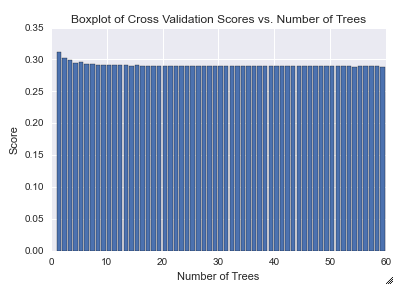
\includegraphics[width=0.7\textwidth]{forest_tuning.png}
\caption{Mean absolute error for 256 features with different sizes of random forest}
\label{my-label}
\end{figure}
Ignoring the slight noise due to randomness, the marginal improvement in predictive power from adding trees to the random forest flattens out around 30 trees, although mean absolute error continues to decrease as the number of trees increases. 
\section*{Feature Selection}
Using rdkit, we generated several new sets of features, which are summarized in Table 1. 
\begin{table}[h]
\centering
\begin{tabular}{|p{4cm}|p{8cm}|p{4cm}|}
\hline
\textbf{Feature Type} & \textbf{Description} & \textbf{Parameters} \\ \hline
Morgan/Circular \newline Fingerprint & Uses the Morgan algorithm to generate a bit \newline vector for each atom and its surrounding \newline neighborhood (defined by parameter radius) & Radius, Number of Bits, Features Invariant \\ \hline
Topological Fingerprint & Identifies and hashes bond paths to generate a bit vector & Number of Bits \\ \hline
MACCS Keys & 166 pre-identified substructures used to generate a fingerprint & None \\ \hline
Chemical Properties & Various binary and nonbinary chemical descriptors for molecules & Features \\ \hline
\end{tabular}
\caption{Summary of various fingerprints and features generated}
\label{my-label}
\end{table}

\subsubsection*{General Strategy}
Our general strategy with feature selection was to generate a large variety of features, then decide quantitatively through cross-validation which features would be most useful for inclusion in our final model. Below we discuss several classes of features that we generated and considered; our final submission, as discussed more in depth in our results section, uses a combination of the Morgan (with and without features) fingerprints and the chemical descriptor features.

\subsubsection*{Morgan/Circular Fingerprint}
The Morgan algorithm generates a bit vector in a given radius around each atom of a molecule. The generated vectors are then hashed to a vector of a user-specified length. \\ \\
\underline{Radius}: The radius parameter defines the size of the atom environment that the algorithm considers when considering each individual atom. A radius of 1, for example, considers the atom and atoms one chemical bond away. Literature suggests that a radius of 2-3 is standard, and through our own cross-validation tests we found that radii above 5 did not significantly improve predictive power. \\ \\
\underline{Number of bits}: Since the Morgan algorithm hashes the results of the analysis of each atom to a bit vector of a specified length, the probability of collision will decrease with a larger number of bits, meaning that we will get a more descriptive fingerprint. We tried vectors of length 256 (as given), 512, and 1024, with cross-validation tests confirming that more bits resulted in better predictions (albeit with decreasing marginal returns). The limiting factor on tuning this parameter was computing power. \\ \\
\underline{Feature-invariant versus atom-invariant}: A parameter that ended up being key to our predictive power was toggling the feature-invariant parameter in rdkit. The first runs we did had the feature-invariant turned on, meaning that the Morgan algorithm looked for pre-defined features based on chemical standards that have proven, in general, to be useful at differentiating molecules. On the other hand, the atom-invariant approach looks for different connectivity information for each atom being considered--number of rings, number of attached hydrogens, etc. \\ \\
As noted in the rdkit documentation \cite{landrum}, these two approaches (feature-invariant, atom-invariant) can sometimes lead to very different similarity scores between the same molecules, and we found that in this case the features that were generated were at least partially orthogonal; in cross-validation tests we saw a marked improvement by concatenating both sets of features and using them as our predictors as opposed to either set alone. The results suggest that the HOMO-LUMO gap is best predicted by some combination of feature and atom invariant features.
\subsubsection*{Topological Fingerprint}
Topological fingerprints identify and hash topological paths to bit vectors. Therefore, as with Morgan Fingerprints, longer bit vectors decrease the probability of collision and allow for more useful fingerprints. The topological features that were identified did not end up outperforming the Morgan features and also did not seem to add any additional predictive power when concatenated with the Morgan feature sets. 
\subsubsection*{MACCS Keys}
Much like the feature-invariant approach in the Morgan Fingerprint, MACCS Keys uses a set of 166 pre-identified substructures as features \cite{dalke}. As it turns out, the rdkit documentation notes that the MACCS Keys and the Morgan feature invariants are based on similar sets of substructures, and so it is not surprising that MACCS failed to outperform even when concatenated with other feature sets. 
\subsubsection*{Chemical Properties}
We considered a variety of chemical descriptors, which includes properties calculated about a molecule based on its molecular structure. Some of these descriptors may have been partially or completely encoded in hashed form via some of the other fingerprint-based methods that we tried, and this correlation may have led to some bias; however, overall, we found that the addition of these chemical descriptor features yielded improvements to our model. The full list of chemical descriptors we considered is listed in this \href{http://www.rdkit.org/docs/GettingStartedInPython.html#list-of-available-descriptors}{RDKit documentation link}. From this list, we extracted 183 features, some of which include molecular weight, number of rings, and various other surface area-related features, such as approximate van der Waals surface area and topological polar surface area. A full list of the features we used can be found in the appendix. The types of data in this feature set, as seen in the appendix, took on a range of values, ranging from binary to integer (such as number of rings, etc.) to continuous variables (such as molecular mass or VSA). \\ \\
Because the rest of our data was binary, we performed LASSO regressions in an attempt to perform feature selection, although we were somewhat confident that our random forest regressor would not overfit or run into huge problems with a mix of continuous and binary data. We also performed this analysis to attempt to see if the most important features as chosen by regularization were reasonable, as these chemical descriptors were more easily mapped to quantities that could be intuitively understood to have some effect on the HOMO-LUMO gap (unlike the fingerprinting results, where the hash made it difficult to tell which feature was impacting which bit). We performed regularization at various $\alpha$ levels, using LASSO due to its shrinkage properties, and found various subsets of the features which seemed to be most important. Specifically, we found a certain subset of features to be useful at the $\alpha = 0.01$ level, which is found in the appendix \hyperlink{alphatable}{here}. We see that some of the most indicative features are the various van der Waals surface area calculations, which make sense intuitively as the size of the surface area in a van der Waals sense help govern the bonding properties and thus the HOMO-LUMO gap. However, as we are not chemists, we simply accept this preliminary eyeball test; in our final run, however, we ended up using all 183 features, as the random forest regressor seemed to be adequately not overfitting the data, even with extraneous features (seen in the table below). We include this discussion of features anyway because the selection of these features as important may lead to some chemical understanding of important features to look at, or may inspire further generation of other similar features which may prove useful even in machine learning approaches.

\begin{table}[H]
\centering
\begin{tabular}{|l|l|l|l|l|}
\hline
\textbf{\begin{tabular}[c]{@{}l@{}}RMSE (100k training)\\ (Mean over 5 runs each)\end{tabular}} & \multicolumn{4}{l|}{\textit{Number of Trees}} \\ \hline
\textit{Chem Features}                                                                          & 30        & 40        & 50        & 60        \\ \hline
None                                                                                            & n/a       & 0.120441  & 0.119135  & n/a       \\ \hline
$\alpha = 0$ (all)                                                                              & 0.116613  & 0.115653  & 0.114607  & 0.114128  \\ \hline
$\alpha = 0.001$                                                                                & 0.116864  & n/a       & n/a       & n/a       \\ \hline
$\alpha= 0.01$                                                                                  & 0.117339  & n/a       & n/a       & n/a       \\ \hline
$\alpha = 0.1$                                                                                  & 0.117965  & n/a       & n/an      & n/a       \\ \hline
\end{tabular}
\caption{RMSE results for various regularization parameters on chemical descriptor feature set}
\label{my-label}
\end{table}

\section*{Results}
Below we present a comprehensive table which document some (but not all) of the training and validation that we considered when deciding which paths to pursue during this practical. Of key importance was the lack of computing power of our team; processing took place on two laptop machines throughout the practical (only two of the laptops owned had sufficient RAM to load the data necessary). Given this constraint, many entries in the testing matrix below are blank due to time constraints. Because of theoretical reasons discussed above, we decided to hone in on one regression model, the random forest regressor, and focus on feature engineering and selection.\\ \\
Here, we present RMSE results in tabular form: across we have various feature sets, and vertically we used various types of regressors. The feature set letters correspond to the following list (separated for readability):

\begin{enumerate}[A:]
\item Morgan fingerprints, radius 1, 256-bit, with features
\item Topological fingerprinting, 1024 bits
\item Morgan fingerprints, radius 2, 512-bit, with features
\item Morgan fingerprints, radius 3, 512-bit, with features
\item Morgan fingerprints, radius 3, 1024-bit, with features
\item Morgan fingerprints, radius 3, 512-bit, no features
\item Combination: Morgan fingerprints, radius 3, 512-bit, features \textit{and} no features
\item Combination: Morgan fingerprints, radius 3, 512-bit, features \textit{and} no features; \textit{and} chemical features
\end{enumerate}

\begin{table}[H]
\centering
\resizebox{\textwidth}{!}{%
\begin{tabular}{|l|l|l|l|l|l|l|l|l|}
\hline
\multicolumn{1}{|c|}{\textbf{Results}} & \multicolumn{8}{c|}{\textit{Feature Set (across)}} \\ \hline
\textit{Method (down)} & A & B & C & D & E & F & G & H \\ \hline
Mean & 0.40682 &  &  &  &  &  &  &  \\ \hline
OLS Regression & 0.29845 &  &  &  &  &  &  &  \\ \hline
SGD Regression (out of the box) & 0.29857 &  &  &  &  &  &  &  \\ \hline
SGD Elastic Net (L1+L2) & 0.29863 &  &  &  &  &  &  &  \\ \hline
Support Vector Regression & 0.29728 &  &  &  &  &  &  &  \\ \hline
\begin{tabular}[c]{@{}l@{}}Random Forest Regression \\ ($K = n_{\textrm{features}}$),\\ 30 trees\end{tabular} & 0.27213 &  &  &  &  &  &  &  \\ \hline
\begin{tabular}[c]{@{}l@{}}Random Forest Regression\\ ($K = \sqrt{n_{\textrm{features}}}$),\\ 30 trees\end{tabular} & 0.27205 & 0.13009 & 0.11343 & 0.10152 & 0.09896 & 0.08201 & 0.07056 & 0.06765 \\ \hline
\begin{tabular}[c]{@{}l@{}}Random Forest Regression\\ ($K = \sqrt{n_{\textrm{features}}}$),\\ 60 trees\end{tabular} &  &  &  &  &  &  &  & 0.06566* \\ \hline
\end{tabular}
}
\caption{Matrix of RMSE results for various feature sets and regressors; (*) is the final submission}
\label{rmse-all}
\end{table}

As can be seen in the above table, we tried various regressors, but decided to focus on the random forest regressor and tuning parameters for that regressor due to limited computational power and due to the attractive features of the random forest as discussed in the body of the paper. Through feature selection improvements, we make gains and eventually come to an RMSE of around 6.6\%. This result held up in the test set, lending credence to our belief about random forests being resilient to overfitting. 

\begin{thebibliography}{}
\bibitem{dalke} Dalke, Andrew. MACCS key 44. Scientific AB, 2013. 
\bibitem{landrum} Landrum, Greg. The RDKit Documentation. 2014. 
\bibitem{loupe} Loupe, Gilles. Understanding Random Forest: From Theory to Practice. University of Liege, 2014. 
\bibitem{pedre} Pedregosa, Fabian, et al. Scikit-learn: Machine Learning in Python. JMLR 12 pp. 2825-2830, 2011. 
\bibitem{steinberg} Steinberg, Dan, Mikhail Golovnya, and N. Scott Cardell. A Brief Overview to Random Forests. Salford Systems, 2004. 
\end{thebibliography}
\section*{Appendix}
\begin{table}[H]
\resizebox{\textwidth}{!}{%
\begin{tabular}{lllll}
BalabanJ                 & NumAromaticHeterocycles  & SlogP\_VSA5          & fr\_alkyl\_halide         & fr\_phenol\_noOrthoHbond \\
BertzCT                  & NumAromaticRings         & SlogP\_VSA6          & fr\_allylic\_oxid         & fr\_phos\_acid           \\
Chi0                     & NumHAcceptors            & SlogP\_VSA7          & fr\_amide                 & fr\_phos\_ester          \\
Chi0n                    & NumHDonors               & SlogP\_VSA8          & fr\_amidine               & fr\_piperdine            \\
Chi0v                    & NumHeteroatoms           & SlogP\_VSA9          & fr\_aniline               & fr\_piperzine            \\
Chi1                     & NumRotatableBonds        & TPSA                 & fr\_aryl\_methyl          & fr\_priamide             \\
Chi1n                    & NumSaturatedCarbocycles  & VSA\_EState1         & fr\_azide                 & fr\_prisulfonamd         \\
Chi1v                    & NumSaturatedHeterocycles & VSA\_EState10        & fr\_azo                   & fr\_pyridine             \\
Chi2n                    & NumSaturatedRings        & VSA\_EState2         & fr\_barbitur              & fr\_quatN                \\
Chi2v                    & PEOE\_VSA1               & VSA\_EState3         & fr\_benzene               & fr\_sulfide              \\
Chi3n                    & PEOE\_VSA10              & VSA\_EState4         & fr\_benzodiazepine        & fr\_sulfonamd            \\
Chi3v                    & PEOE\_VSA11              & VSA\_EState5         & fr\_bicyclic              & fr\_sulfone              \\
Chi4n                    & PEOE\_VSA12              & VSA\_EState6         & fr\_diazo                 & fr\_term\_acetylene      \\
Chi4v                    & PEOE\_VSA13              & VSA\_EState7         & fr\_dihydropyridine       & fr\_tetrazole            \\
EState\_VSA1             & PEOE\_VSA14              & VSA\_EState8         & fr\_epoxide               & fr\_thiazole             \\
EState\_VSA10            & PEOE\_VSA2               & VSA\_EState9         & fr\_ester                 & fr\_thiocyan             \\
EState\_VSA11            & PEOE\_VSA3               & fr\_Al\_COO          & fr\_ether                 & fr\_thiophene            \\
EState\_VSA2             & PEOE\_VSA4               & fr\_Al\_OH           & fr\_furan                 & fr\_unbrch\_alkane       \\
EState\_VSA3             & PEOE\_VSA5               & fr\_Al\_OH\_noTert   & fr\_guanido               & fr\_urea                 \\
EState\_VSA4             & PEOE\_VSA6               & fr\_ArN              & fr\_halogen               &                          \\
EState\_VSA5             & PEOE\_VSA7               & fr\_Ar\_COO          & fr\_hdrzine               &                          \\
EState\_VSA6             & PEOE\_VSA8               & fr\_Ar\_N            & fr\_hdrzone               &                          \\
EState\_VSA7             & PEOE\_VSA9               & fr\_Ar\_NH           & fr\_imidazole             &                          \\
EState\_VSA8             & RingCount                & fr\_Ar\_OH           & fr\_imide                 &                          \\
EState\_VSA9             & SMR\_VSA1                & fr\_COO              & fr\_isocyan               &                          \\
FractionCSP3             & SMR\_VSA10               & fr\_COO2             & fr\_isothiocyan           &                          \\
HallKierAlpha            & SMR\_VSA2                & fr\_C\_O             & fr\_ketone                &                          \\
HeavyAtomCount           & SMR\_VSA3                & fr\_C\_O\_noCOO      & fr\_ketone\_Topliss       &                          \\
Ipc                      & SMR\_VSA4                & fr\_C\_S             & fr\_lactam                &                          \\
Kappa1                   & SMR\_VSA5                & fr\_HOCCN            & fr\_lactone               &                          \\
Kappa2                   & SMR\_VSA6                & fr\_Imine            & fr\_methoxy               &                          \\
Kappa3                   & SMR\_VSA7                & fr\_NH0              & fr\_morpholine            &                          \\
LabuteASA                & SMR\_VSA8                & fr\_NH1              & fr\_nitrile               &                          \\
MolLogP                  & SMR\_VSA9                & fr\_NH2              & fr\_nitro                 &                          \\
MolMR                    & SlogP\_VSA1              & fr\_N\_O             & fr\_nitro\_arom           &                          \\
NHOHCount                & SlogP\_VSA10             & fr\_Ndealkylation1   & fr\_nitro\_arom\_nonortho &                          \\
NOCount                  & SlogP\_VSA11             & fr\_Ndealkylation2   & fr\_nitroso               &                          \\
NumAliphaticCarbocycles  & SlogP\_VSA12             & fr\_Nhpyrrole        & fr\_oxazole               &                          \\
NumAliphaticHeterocycles & SlogP\_VSA2              & fr\_SH               & fr\_oxime                 &                          \\
NumAliphaticRings        & SlogP\_VSA3              & fr\_aldehyde         & fr\_para\_hydroxylation   &                          \\
NumAromaticCarbocycles   & SlogP\_VSA4              & fr\_alkyl\_carbamate & fr\_phenol                &                         
\end{tabular}
}
\caption{List of chemical features used}
\end{table}

\begin{table}[H]
\centering
\begin{tabular}{lll}
BertzCT      & PEOE\_VSA14 & SlogP\_VSA1       \\
EState\_VSA2 & PEOE\_VSA3  & SlogP\_VSA12      \\
EState\_VSA3 & PEOE\_VSA4  & SlogP\_VSA2       \\
EState\_VSA4 & PEOE\_VSA5  & SlogP\_VSA3       \\
EState\_VSA5 & PEOE\_VSA7  & SlogP\_VSA5       \\
EState\_VSA6 & PEOE\_VSA8  & SlogP\_VSA6       \\
EState\_VSA8 & PEOE\_VSA9  & TPSA              \\
EState\_VSA9 & SMR\_VSA10  & VSA\_EState9      \\
MolMR        & SMR\_VSA3   & fr\_allylic\_oxid \\
PEOE\_VSA1   & SMR\_VSA7   & fr\_bicyclic      \\
PEOE\_VSA11  & SMR\_VSA9   & fr\_pyridine     
\end{tabular}
\caption{Features selected by LASSO at $\alpha = 0.01$ level.}
\end{table}
\hypertarget{alphatable}{}


\end{document}
